\documentclass[a4paper]{article}

\usepackage[T1]{fontenc}	
\usepackage{amsmath}
\usepackage{amssymb}
\usepackage{graphicx}
\usepackage{fancyhdr}

\pagestyle{fancy}
\lhead{Computer Excercise 1}
\rhead{Kristoffer Nordström, Noah Hansson}
\cfoot{\thepage}

\title{Computer Exercise 1 - NEKN83}
\author{Kristoffer Nordström, Noah Hansson}
\date{\today}


\begin{document}

\maketitle

\section{Introduction}
The purpose of this exercise \ref{var1}

\section{Empirical Results}

\begin{figure}
    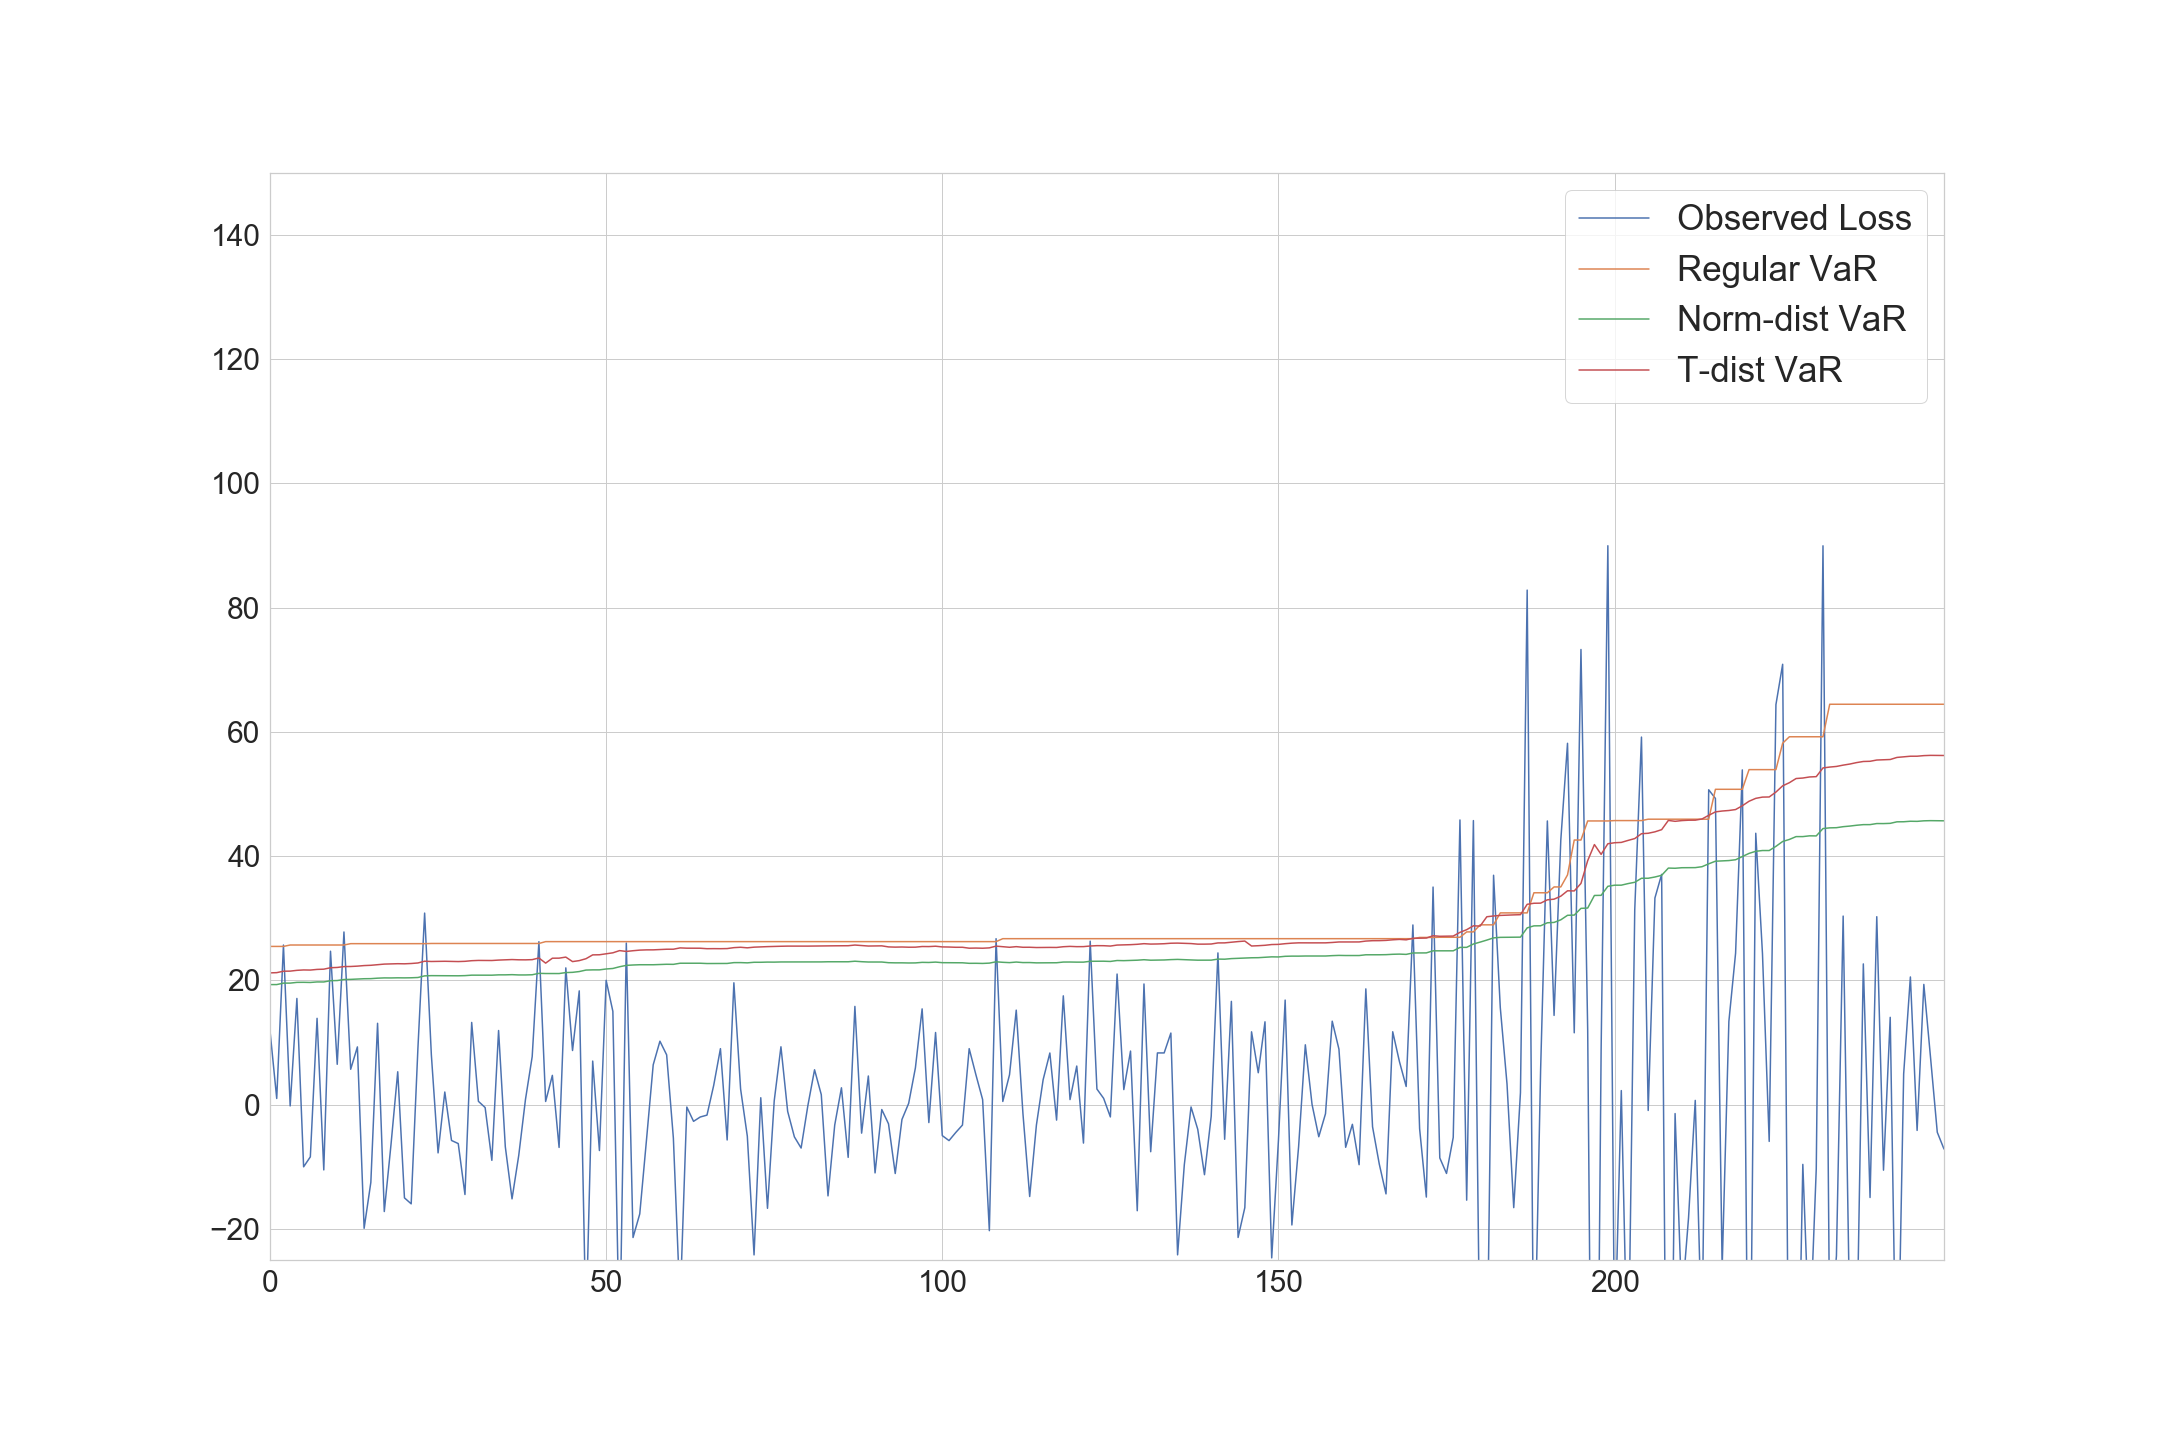
\includegraphics[width=\textwidth]{VaR1.png}
    \caption{Observed loss compared to $VaR_{99\%}$ estimates based on historical volatility}
    \label{var1}
\end{figure}

\begin{figure}
    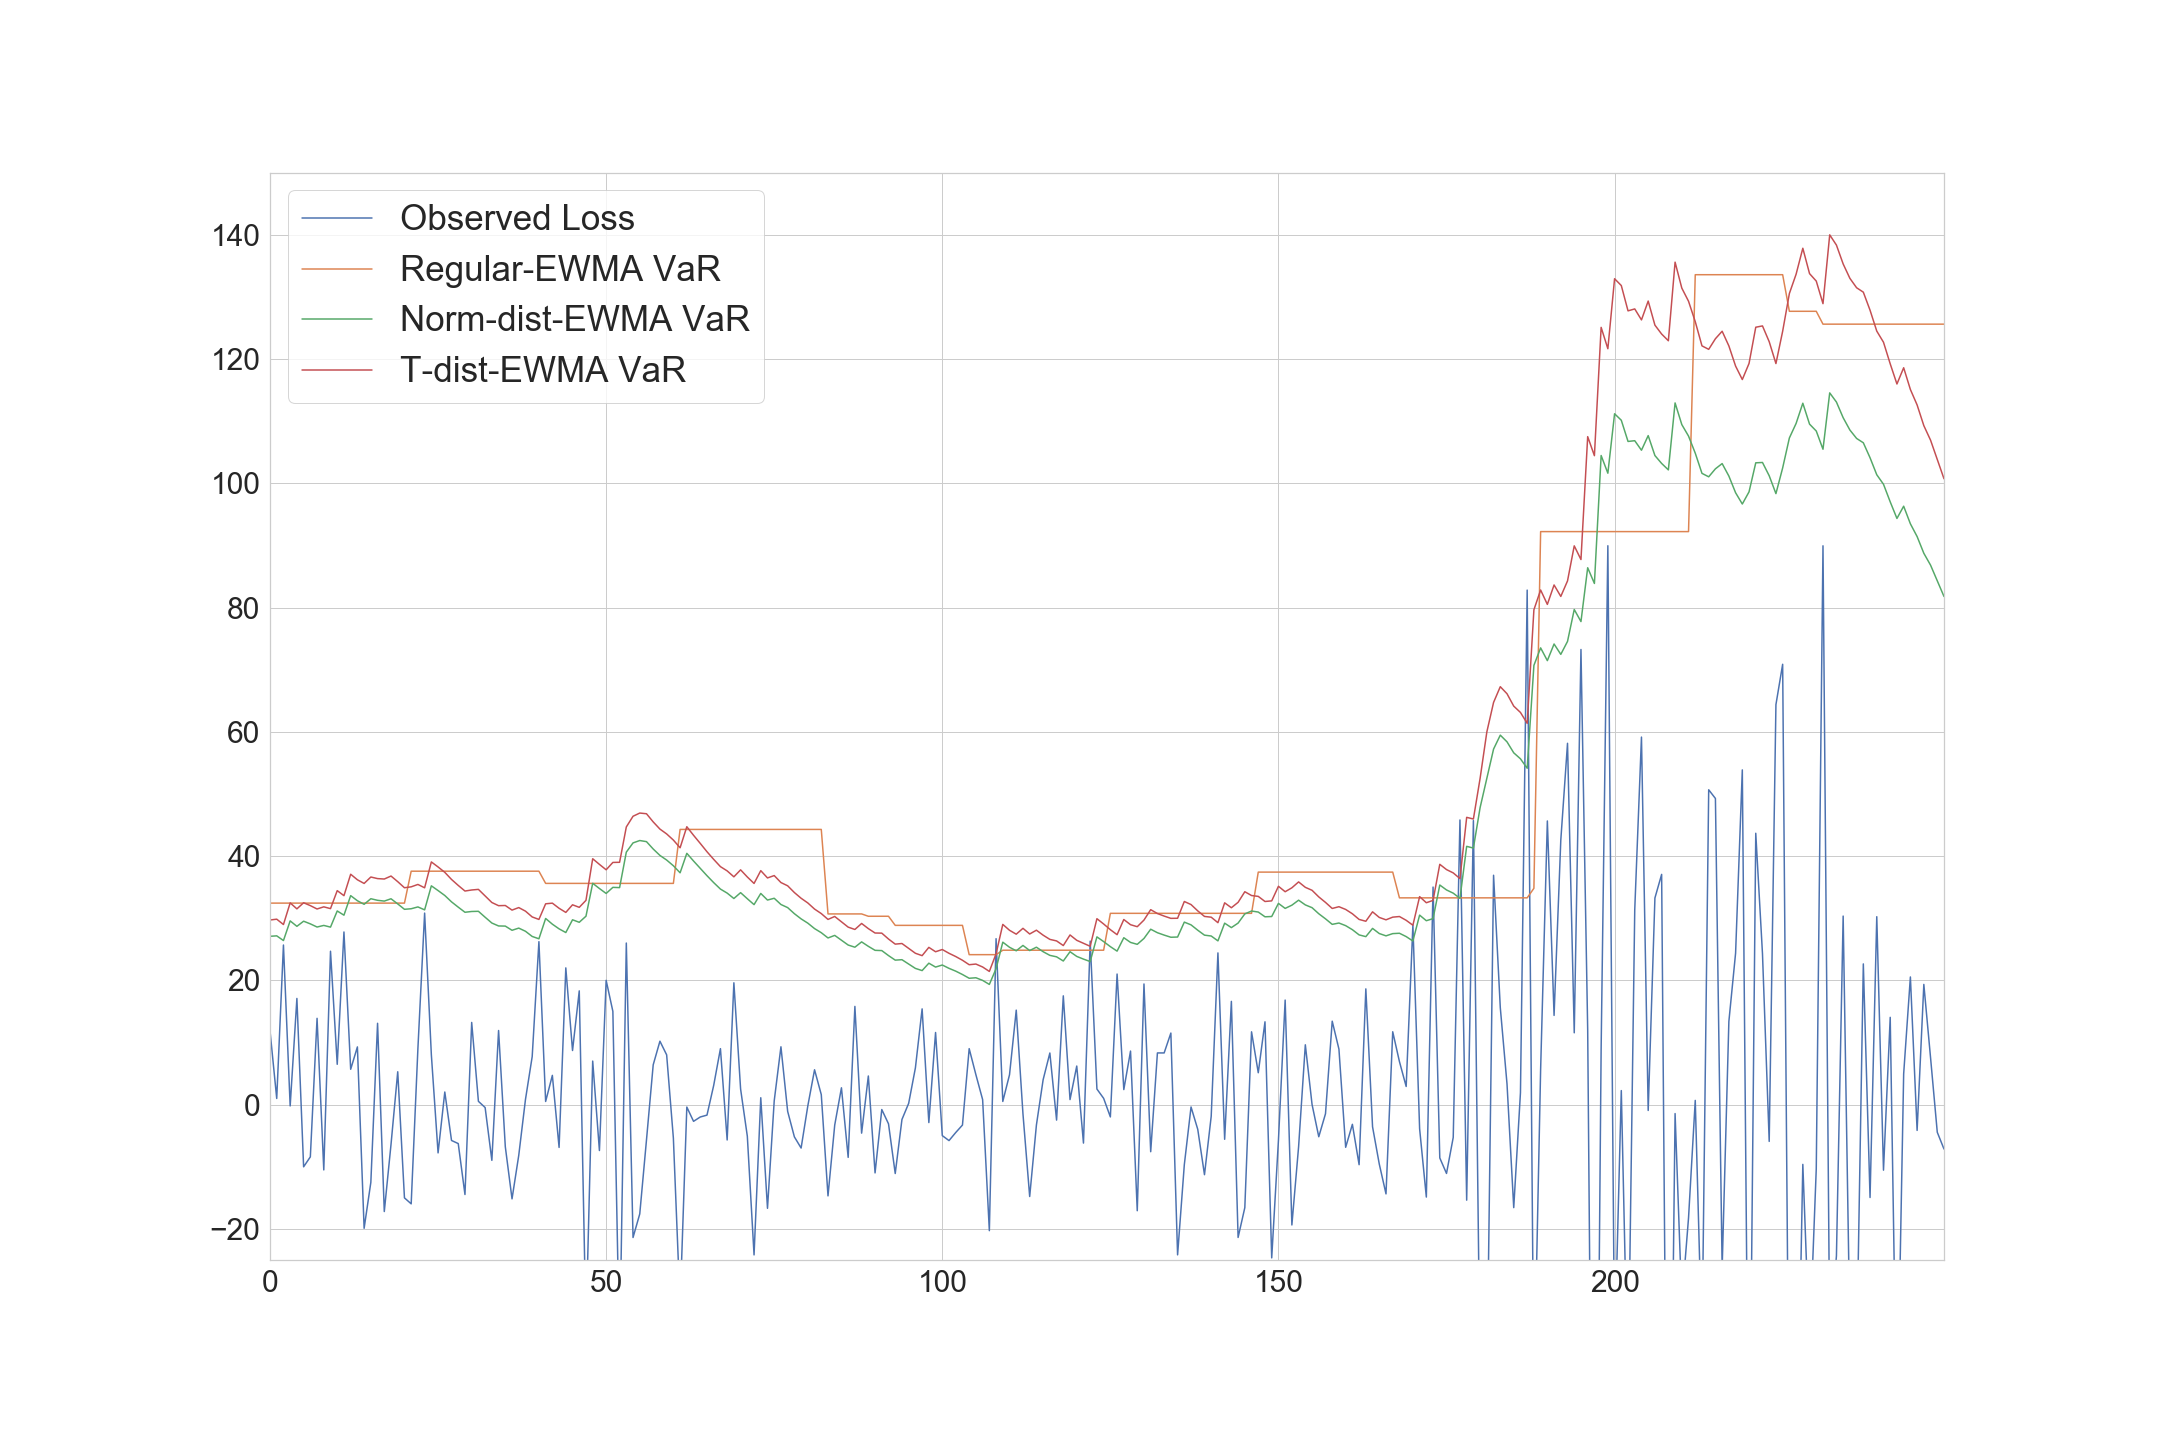
\includegraphics[width=\textwidth]{VaR2.png}
    \caption{Observed loss compared to $VaR_{99\%}$ estimates based on EWMA volatility predictions}
    \label{var2}
\end{figure}

\section{Conclusion}
As seen when comparing figure \ref{var1} and figure \ref{var2}, using an EWMA volatility predictor gives us a better VaR-estimate. In fact, the only VaR estimate that manages to pass the Kupiec test is the EWMA T-distribution estimate. However, both methods have their pros and cons. Even though the EWMA methods better manage to follow the market when volatility spikes, it also has a higher variance in estimates, and tends to over-react some times. This gives a higher VaR-estimate than necessary. When volatility is rather constant the historical volatility estimates give a lower VaR without causing too many violations. \newline
We can also see that the choice of volatility model matters a lot more than the underlying assumption of distribution of the loss function. As such, the first step towards making a more reliable estimator would be to find a better predictor of volatility.

\end{document}
